\subsection{Quelques exemples}


Obsolescences technologiques

\paragraph*{obsolescence d’incompatibilité logiciel :}

cf \ref{compSamsIph}
\begin{figure}[h]

\begin{minipage}{0.5\linewidth}
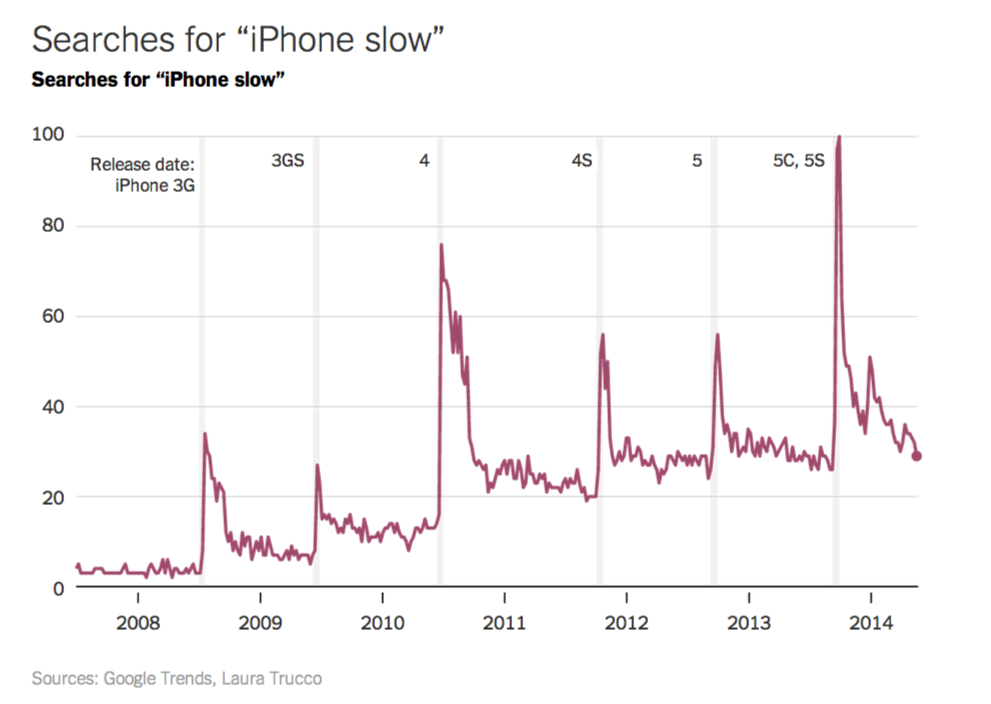
\includegraphics[scale=0.25]{Rsc/searchForIphoneSlow.png} 
\end{minipage}
\begin{minipage}{0.5\linewidth}
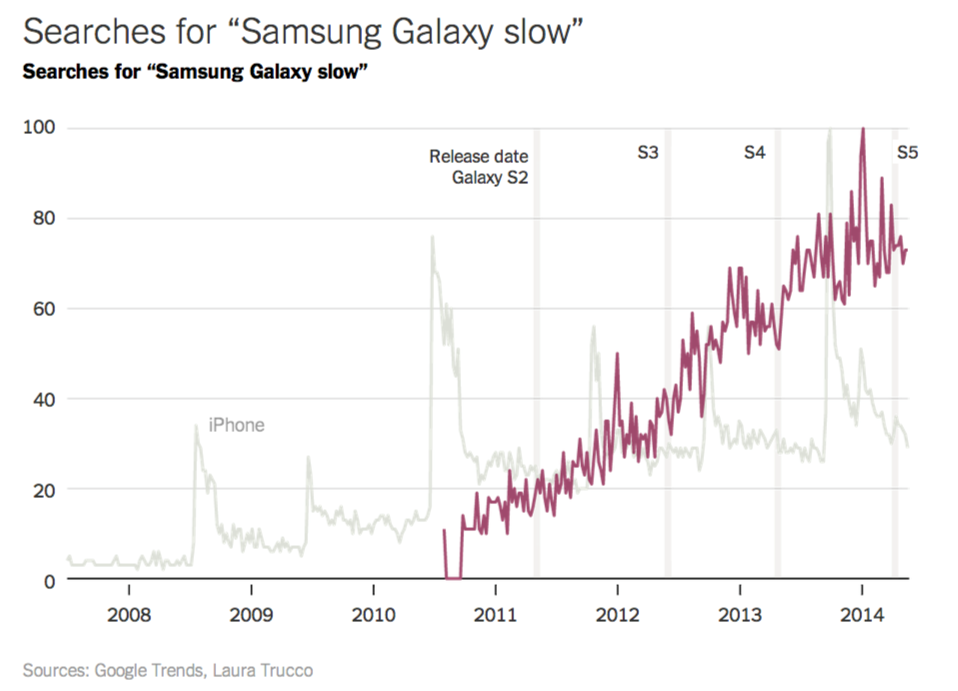
\includegraphics[scale=0.25]{Rsc/searchForSamsungSlow.png} 
\end{minipage}
\caption{Comparaison entre samsung et iPhone}
\label{compSamsIph}
\end{figure}

\paragraph*{obsolescence indirect :}

Malgré la norme USB imposée par l’union européenne, Apple utilise toujours ses propres connecteurs, et ne manque pas de changer la forme du connecteur d’une génération à une autre pour rendre obsolètes les anciens modèles.

\paragraph*{obsolescence de fonctionnement :}

Les batteries d’ipod étaient irremplaçables pour les 1ere, 2eme et 3eme générations. Un procès a été intenté par Elizabeth Pritzyker, ce qui a conduit Apple à mettre en place une politique de remplacement des batteries usées.

\paragraph*{Obsolescence de service après-vente :}

Le 8 avril 2014, Microsoft annonce la fin du service après-vente du système d’exploitation Windows XP, encore très présent en entreprise. Que ce soit pour pousser au rachat d’un système de génération plus récente ou pour se décharger de la responsabilité de certaines failles, cette décision met en péril la sécurité de plus de 20% des terminaux mondiaux. Aux États-Unis 95% des distributeurs de billets du pays fonctionnaient encore sous XP en janvier 2014.



\paragraph*{Obsolescence psychologique :}

Grâce à l’extrait d’ACV fourni à GreenIT.fr par Fujitsu, on apprend que le bilan carbone de production peut être jusqu’à 70 fois supérieur au bilan carbone d’utilisation pour un ordinateur fabriqué en Asie. Il faut prendre en compte le fait que la Chine utilise abondamment le charbon dans sa production d'électricité. Pour cette raison il est important de mesurer les arguments écologiques des produits mis en vente, avant de remplacer un appareil qui fonctionne encore. De même les effets de mode poussent à remplacer des produits totalement fonctionnels.
